Considera la funció
\[
f(x)=\begin{cases}
  x^2 & \si{x\le 1},\\[4pt]
  2-\dfrac{1}{x} & \si{x>1}.
\end{cases}
\]

\begin{apartats}

\apartat[1,25]{1}
Estudia'n la continuïtat i troba'n les asímptotes.

\begin{solucio}
Cada branca és contínua al seu tros, i en $x=1$: $f(1)=1$, $\lim_{x\to1^-}f(x)=1$ i
$\lim_{x\to1^+}f(x)=2-1=1$. La funció és \textbf{contínua a tot $\mathbb{R}$}.\\
\textbf{Asímptotes verticals}: no n'hi ha. L'únic punt problemàtic de la segona branca seria
$x=0$, que no és al seu tros.\\
\textbf{Horitzontals}: $\lim_{x\to+\infty}f(x)=2$, i per tant $y=2$ és asímptota horitzontal
per la dreta. Per l'esquerra, $\lim_{x\to-\infty}x^2=+\infty$: no n'hi ha.
\end{solucio}

\begin{nomesllarg}
\apartat{0,75}
Estudia'n la monotonia i troba'n els extrems.

\begin{solucio}
Per a $x<1$: $f'(x)=2x$, negativa a $(-\infty,0)$ i positiva a $(0,1)$.\\
Per a $x>1$: $f'(x)=\dfrac{1}{x^2}>0$, sempre creixent.\\
Així, $f$ \textbf{decreix} a $(-\infty,0)$ i \textbf{creix} a $(0,+\infty)$: hi ha un
\textbf{mínim} en $(0,0)$, que a més és el mínim absolut.
\end{solucio}
\end{nomesllarg}

\apartat[1,25]{0,75}
Representa la funció.

\begin{solucio}
A l'esquerra de $x=1$ és la paràbola $y=x^2$; a la dreta, una branca creixent que s'acosta a
$y=2$ sense arribar-hi. Les dues branques s'enganxen en $(1,1)$.
\begin{center}
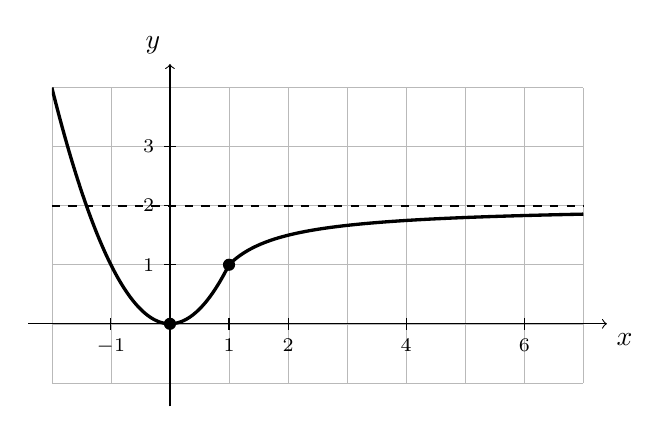
\begin{tikzpicture}[x=0.75cm,y=0.75cm]
  \draw[gray!55,very thin,step=1] (-2,-1) grid (7,4);
  \draw[->] (-2.4,0) -- (7.4,0) node[below right] {$x$};
  \draw[->] (0,-1.4) -- (0,4.4) node[above left] {$y$};
  \foreach \i in {-1,1,2,4,6} \draw (\i,0.1) -- (\i,-0.1) node[below,font=\scriptsize] {$\i$};
  \foreach \j in {1,2,3} \draw (0.1,\j) -- (-0.1,\j) node[left,font=\scriptsize] {$\j$};
  \draw[dashed,thick] (-2,2) -- (7,2);
  \begin{scope}
    \clip (-2,-1) rectangle (7,4);
    \draw[\colorgrafica,very thick,domain=-2:1,samples=60,smooth] plot (\x,{\x*\x});
    \draw[\colorgrafica,very thick,domain=1:7,samples=100,smooth] plot (\x,{2-1/\x});
  \end{scope}
  \fill (1,1) circle (2.2pt); \fill (0,0) circle (2.2pt);
\end{tikzpicture}
\end{center}
\end{solucio}

\end{apartats}
